\subsection{Ordini}
Gli ordini di una CP-Net, come è noto, sono delle informazioni che
consentono di determinare tra due assegnamenti alle variabili del
problema, nel contesto della semantica dei flip peggiorativi, quale
delle due rappresenti un'assegnamento maggiormente preferito.

Le informazioni irrinunciabili per costruire un ordine sono:
\begin{itemize}
\item Il nome della variabile (e quindi il corrispondente dominio) cui
  l'ordine si riferisce,
\item L'elenco delle eventuali dipendenze,
\item Una mappa che associ ad ogni assegnamento delle variabili di
  dipendenza un ordine totale degli elementi della variabile.
\end{itemize}

La rappresentazione in memoria che è stata scelta per gli ordini è una
struttura dati ad albero. Il motivo di tale scelta risiede nel fatto
che l'utilità dell'ordine è inversamente proporzionale alla quantità
di tempo necessario per indivduare quale è l'ordinamento dei valori
della variabile nel contesto di un certo assegnamento delle variabili
di dipendenza. Date le caratteristiche delle CPNet (a)cicliche è
infatti evidente che se una variabile A dipende dalle variabili B, C e
D, allora la quantità complessiva di ordini totali degli elementi di A
è esattamente pari a $ |dom(B)| \cdot |dom(C)| \cdot |dom(D)| $. La
ricerca di un ordine particolare richiederebbe l'individuazione di una
tupla di elementi di B, C e D all'interno di una struttura dati e la
soluzione che si è adotatta consente di avere un occupazione di
memoria, nell'esempio in esame, di $ O(|dom(A)| \cdot |dom(B)| \cdot
|dom(C)| \cdot |dom(D)|)$ (la minima necessaria per memorizzare un
ordine - $ O(|dom(A)|) $ - per ogni possibile tupla - $ O(|dom(B)|
\cdot |dom(C)| \cdot |dom(D)|)$), e un tempo di ricerca di un ordine
di $O(|dom(A)|+|dom(B)|+|dom(C)|+|dom(D)|)$ (tuttavia migliorabile ad
$O(1)$ come risulterà chiaro dalle sezioni successive).

\subsubsection{Struttura ad albero}
Nella rappresentazione ad albero utilizzata, a ciascun livello di
profondità dalla radice è associata una variabile da cui dipende la
variabile dell'ordine. Nell'esempio presentato nella sezione
precedente, la variabile B sarebbe associata alla profondità 0, la
variabile C alla profondità 1 e la variabile D alla profondità
2. L'ordine in cui una variabile è associata ad una profondità non è
rilevante in termini di prestazioni.

In corrispondenza della profondità associata a ciascuna variabile di
dipendenza, si trovano sempre dei \emph{nodi interni} mentre alla
profondità massima si trovano solo \emph{nodi foglia}. Ad un nodo
interno di profondità \emph{i} è memorizzato un array contenente tutti
i valori che la variabile associata al livello di profondità \emph{i}
può assumere e un puntatore al successivo nodo dell'albero associato a
tale assegnamento. Ad un nodo foglia è associato invece un ordine,
rappresentato come mappa tra stringhe e interi, che interessa la
variabile dell'ordine. Il principio di funzionamento si basa sul fatto
che per arrivare ad un nodo foglia di profondità $n+1$, è necessario
seguire i puntatori di $n$ nodi interni memorizzati assieme a dei
valori assunti dalla variabile associata a ciascun livello di
profondità; l'ordine contenuto in tale nodo foglia è quindi quello
associato al contesto ricostruito dalla radice all'ultimo nodo
interno, assegnando ad ogni variabile di ogni livello di profondità il
valore seguito per costruire il cammino.

Ad esempio, sia $dom(A)=\{a, \overline{a}\}$, $dom(B)=\{b,
\overline{b}\}$, $dom(C)=\{c, \overline{c}\}$, $dom(D)=\{d,
\overline{d}\}$. Per rappresentare gli ordini di A nel caso in cui A
dipenda da B, C e D la struttura a grafo sarà la seguente.

\begin{center}
  \begin{figure}[ht]
    \centering
    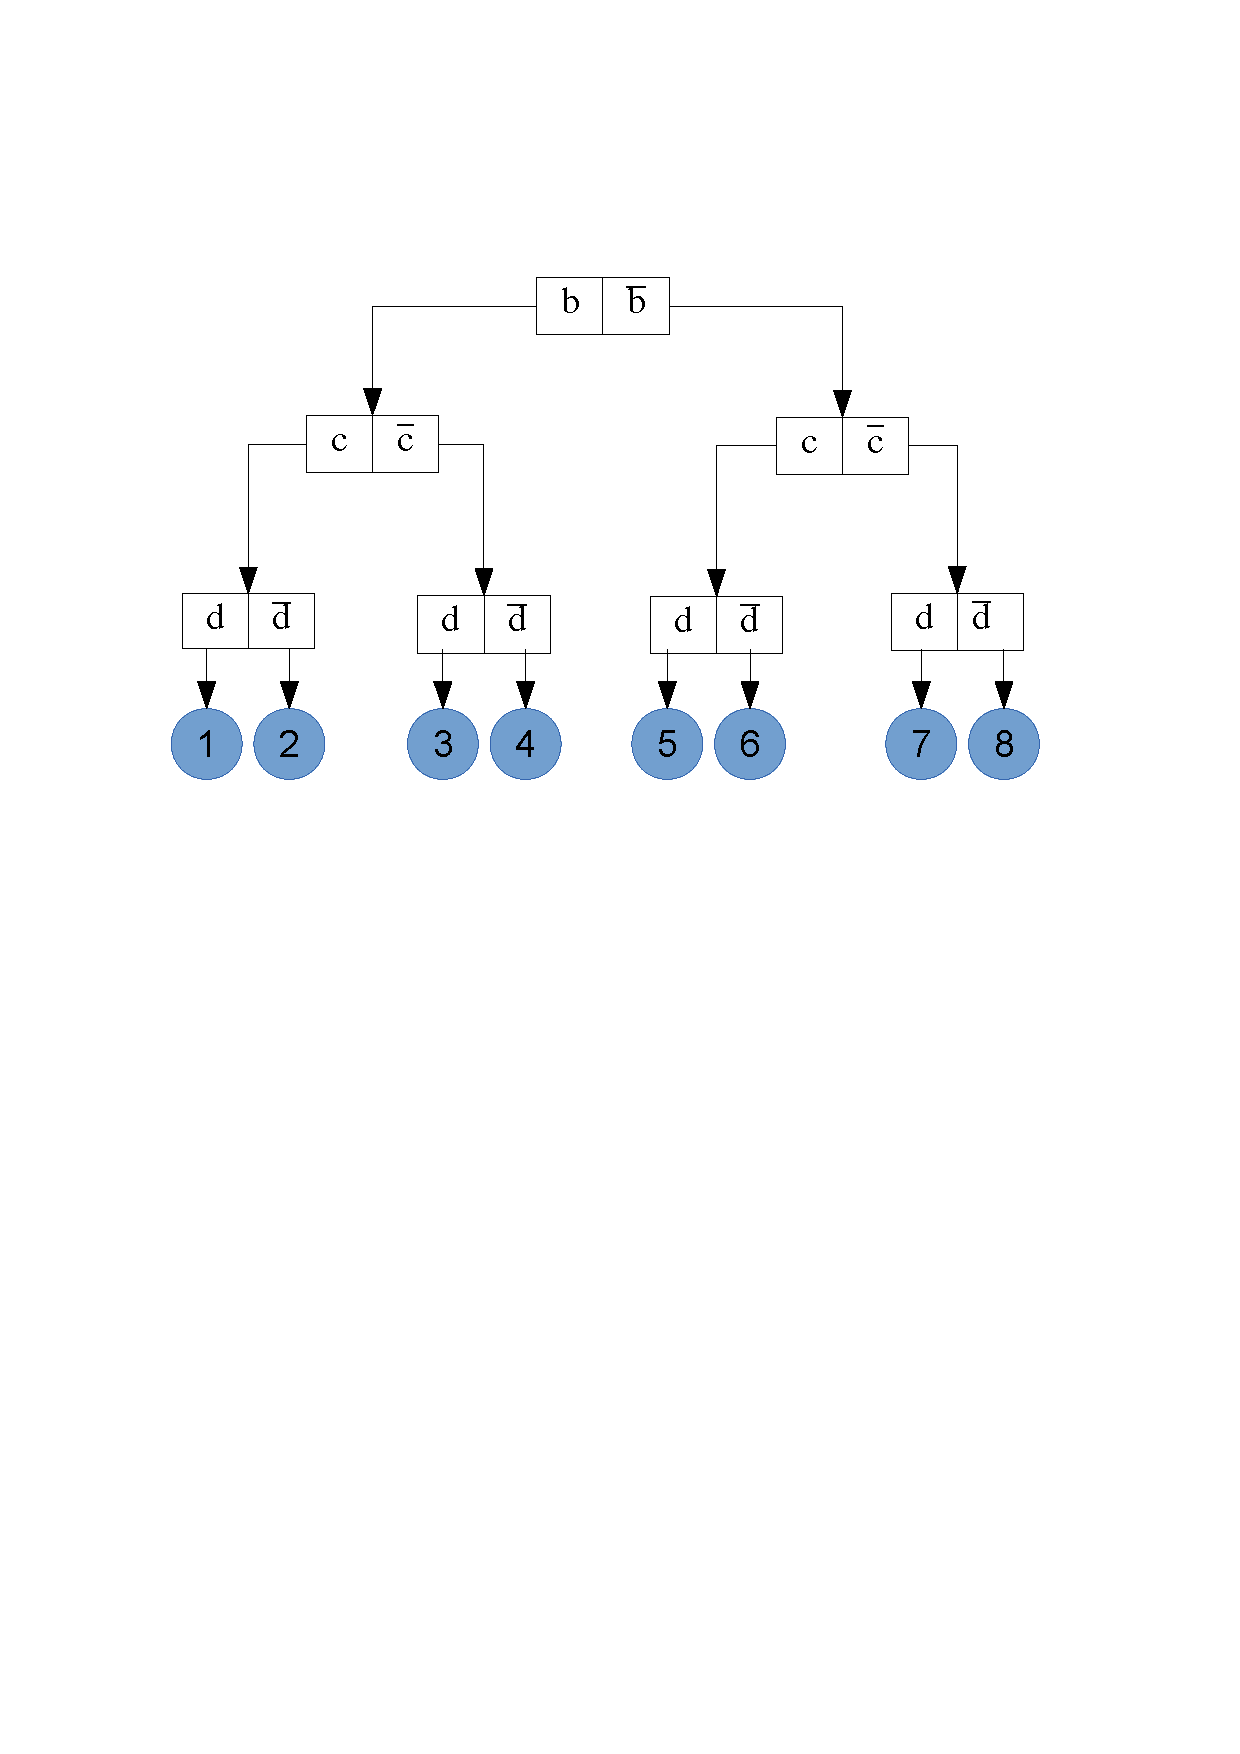
\includegraphics[width=0.5\textwidth]{grafo-ordini}
    \caption{\textit{Rappresentazione a grafo di A, B, C, D}}
  \end{figure}
\end{center}

Nell'esempio si vede chiaramente che per raggiungere ciascuno degli
ordini - ivi rappresentati con dei nodi azzurri numerati - è
necessario costruire un cammino a partire dalla radice alla foglia
relativa all'ordine che equivale ad un assegnamento alle variabili (ad
esempio per raggiungere l'ordine associato ad A identificato con 5 è
necessario assegnare $B=\overline{b}, C=c, D=\overline{d}$).

\subsubsection{Inizializzazione}
Per poter inserire gli ordini è innanzitutto necessario avere a
disposizione la struttura interna dell'albero in cui poi poter
inserire le foglie. Dato che per avere a disposizione una CP-Net
valida è necessario avere tutti gli ordini associati agli assegnamenti
delle variabili di dipendenza, è evidente che sia possibile
inizializzare dapprincipio l'intera struttura interna nel momento in
cui si costruisce l'ordine. Tale struttura infatti dipende unicamente
dalle variabili di dipendenza e dai loro elementi e non è necessaria
alcuna informazione sugli ordini alle foglie per poterla costruire.

All'interno del progetto questa inizializzazione viene effettuata alla
costruzione degli oggetti ordini e la complessità della costruzione è
pari a $O(|dom(V_1)| \cdot \dots \cdot |dom(V_n)|)$ ove $ V_1, \dots,
V_n $ sono tutte le variabili di dipendenza dell'ordine.

\subsubsection{Complessità}
Vista la rappresentazione è quindi evidente che la complessità della
ricerca di un assegnamento $ V_1=v_1, \dots, V_n=v_n $ dipenda da:

\begin{itemize}
\item numero di variabili di dipendenza (n) che comunque si può
  assumere come costante in quanto una volta costruito l'ordine tale
  parametro non cambia mai,
\item ricerca del valore $v_i$ all'interno del nodo interno
  \textit{i-esimo}
\end{itemize}

Dovrebbe risultare quindi evidente che la rappresentazione dei valori
assunti da ogni variabile nei nodi interni determina la complessità
della ricerca. Detta $W$ la variabile a dominio di cardinalità massima
allora
\begin{itemize}
\item se i dati sono memorizzati come array non ordinato allora la
  complessità della ricerca sarà pari a $O(n \cdot
  |dom(W)|)=O(|dom(W)|)$.
\item se i dati sono memorizzati in una struttura dati ordinata allora
  la complessità della ricerca sarà pari a $O(n \cdot
  log|dom(W)|)=O(log|dom(W)|)$.
\item se i dati sono memorizzati in una tabella hash (facile da
  costruire dato che si sa fin dal principio quanti elementi inserire)
  allora la complessità della ricerca sarà pari a $O(n \cdot
  1)=O(n)=O(1)$.
\end{itemize}

\subsubsection{Comparatori}
\label{sect:comparatori}
I Comparatori sono oggetti associati ad un ordine che sono
utilizzabili per costruire la semantica dei flip peggiorativi. L'idea
è che dato un ordine si ha a disposizione l'albero associato a tale
ordine e quindi è facile riuscire a determinare quale è il migliore
tra due assegnamenti che differiscono per un solo valore associato
alla medesima variabile.

Dati gli assegnamenti $X=(V_1=v_1, \dots, V_{i-1}=v_{i-1}, V_i=x,
V_{i+1}=v_{i+1}, \dots, V_m=v_m)$ e $Y=(V_1=v_1, \dots,
V_{i-1}=v_{i-1}, V_i=y, V_{i+1}=v_{i+1}, \dots, V_m=v_m)$\footnote{$m$
  è usato per indicare il numero di variabili del problema} un
comparatore di un ordine associato alla variabile $V_i$ procede come
segue:
\begin{enumerate}
\item Accetta sequenzialmente tutti gli assegnamenti $V_1=v_1, \cdots,
  V_{i-1}=v_{i-1}, V_{i+1}=v_{i+1}, \dots, V_m=v_m)$.
\item Non appena tutte le variabili da cui dipende $V_i$ sono state
  fornite, il comparatore scandisce l'albero dell'ordine di $V_i$ fino
  trovare l'ordine associato all'assegnamento.
\item Trovato l'ordine associato, il comparatore può rispondere al
  confronto tra $x$ e $y$ perché dispone di tutte le informazioni: è
  sufficiente confrontare i valori associati alla mappa dell'ordine a
  $x$ e $y$ per sapere quale dei due è migliore dell'altro.
\end{enumerate}